%
% File acl2020.tex
%
%% Based on the style files for ACL 2020, which were
%% Based on the style files for ACL 2018, NAACL 2018/19, which were
%% Based on the style files for ACL-2015, with some improvements
%%  taken from the NAACL-2016 style
%% Based on the style files for ACL-2014, which were, in turn,
%% based on ACL-2013, ACL-2012, ACL-2011, ACL-2010, ACL-IJCNLP-2009,
%% EACL-2009, IJCNLP-2008...
%% Based on the style files for EACL 2006 by 
%%e.agirre@ehu.es or Sergi.Balari@uab.es
%% and that of ACL 08 by Joakim Nivre and Noah Smith

\documentclass[11pt,a4paper]{article}
\usepackage[hyperref]{acl2020}
\usepackage{booktabs}
\usepackage{graphicx}
\usepackage{times}
\usepackage{latexsym}
\renewcommand{\UrlFont}{\ttfamily\small}

\usepackage{microtype}

\aclfinalcopy % Uncomment this line for the final submission


\newcommand\BibTeX{B\textsc{ib}\TeX}

\title{Digital Socrates: Classifying Action Statements as (Un)Ethical}

\author{Harper Lyon \\
  Tulane University / New Orleans, LA \\
  \texttt{hlyon@tulane.edu}}

\date{}

\begin{document}
\maketitle

\section{Problem Overview}

The idea of ethical machines is attractive, but challenging to implement in practice. One approach is to borrow techniques from sentiment analysis \cite{hendrycks2023aligning} to classify everyday descriptions of actions as ethical or not, creating ideally a system which can give human-like responses to human questions about decisions. This problem contains many of the same inherent challenges as sentiment analysis, as subtle differences in language use can shift the meaning of documents massively - consider the difference between "I will not break my promise even for money" and "I will not break my promise except for even more money" - but also in that it seemingly requires more modeling of meaning than simple sentiment analysis, since ethical judgements are inherently tied to actions in a way that movie reviews or teaching evaluations are not. 

The "hook" for my project is the creation of a webpage where a digital facsimile of Socrates, the famously wise and annoying Athenian, tells you whether or not what you are planning to do is ethical, but for that I will need a classification model capable of accurately making that decision.

\section{Data}

My primary data source is the ETHICS \cite{hendrycks2023aligning} dataset, which is a dataset combining five semi-distinct text classification tasks related to various areas of ethical reasoning. For my purposes, only two subsections of the dataset are useful, and these are as follows:

\begin{table}[htbp]
    \centering
    \caption{Dataset Divisions}
    \begin{tabular}{llll}
        \toprule
        & \textbf{Rows} & \textbf{Classes}\\
        \midrule
        Commonsense & $21.8$k & $0:11.49$k, $1:10.26$k\\
        Justice & $26.5$k & $0:12.31$k, $1:14.23$k\\
        \bottomrule
    \end{tabular}
    \label{tab:my_table}
\end{table}

These two subsets are similar, but not exactly the same. The commonsense dataset consists of two types of document class pairs, the first being straightforward action descriptions 
like ("I left her bleeding on the snowy hillside.", 1) and the other being posts sourced from reddit.com/r/AITAH, an internet forum where users post stories from their lives and receive crowdsourced moral judgements. We can question of the wisdom of relying on these judgements, but they are a convinient corpus for this project. 

The justice dataset consists of statements of the for I (deserve/did) \textit{action} because \textit{reason}, for example ("I deserve to get a nice haircut from my barber because I paid him to make my hair look nice.", 1). Some work is required to reconcile these datasets to a single task - mainly switching the labels to match - I see no reason that they cannot be accomplished by the same model or at least by similar models trained in similar ways.

I am also in the early stages of finding additional data sources to augment my training data, more information on those potential sources \cite{lourie2021scruples}\cite{ziems2022moral} in Related Work.

\section{Methods}

My goal is to evaluate three distinct approaches to this task at different "weights", in particular

\begin{enumerate}
    \item Logistic Regression
    \item Finetuned BERT
    \item Llama
\end{enumerate}

Logistic regression serves as a baseline model, since it will ultimately work through simple word inclusion, but it should give us a good idea, more or less, of how difficult the task is. Otherwise I don't expect it to be all that interesting or play a large part in my final application.

Much of the existing work in this area focuses on BERT based models \cite{lourie2021scruples}\cite{hendrycks2023aligning}, so these are a natural place to begin the real work. There are many BERT varieties, so I expect to try several options (currently I have only worked with distilbert). However, the best BERT based performance so far outside of the commonsense data subset is moderate at best, with ALBERT\cite{lan2020albert} achieving $59.9\%$ on the justice task and $85.5\%$ on commonsense. I don't expect to beat those numbers given my limited resources and time, but it's clear that especially on justice BERT is not up to the task of top notch performance.

What I really want to explore is using an LLM like Llama to generate classifications since this is an area left open by the originators of the ETHICS dataset. I plan to use Llama-2-7b since I am limited by computing power, and that is the most moderate of the new models available. I have already been given access by Meta to the weights for this model, so I will be beginning work here soon.

Evaluation will be straightforward, I am interested in achieving high accuracy and not much else. If I can match the median results of the original paper I'll be happy with my outcomes. I'm also interested in examining the loss variance

\section{Preliminary Results}

So far I have (on the commonsense subset only) implemented the Logistic Regression model and made a first clumsy pass at finetuning a BERT variant called DistilBERT \cite{sanh2020distilbert}, which I chose for no other reason than that is quick to train as a proof of concept and seems to be the "standard" BERT variant used for classification absent other considerations. I've achieved extremely poor performance with both models, hitting exactly chance on Logistic Regression (recall that we have a 50/50 class split) for Logistic Regression \ref{fig:log_reg} and actually performing worse than chance with DistilBERT \ref{fig:distil}. I'm not surprised by the results of logistic regression, but I am disappointed at how poorly DistilBERT performed - there is definitely an over-fitting or analogous issue since the model acheived ~$85\%$ accuracy on the validation split.

\begin{figure}
  \centering
  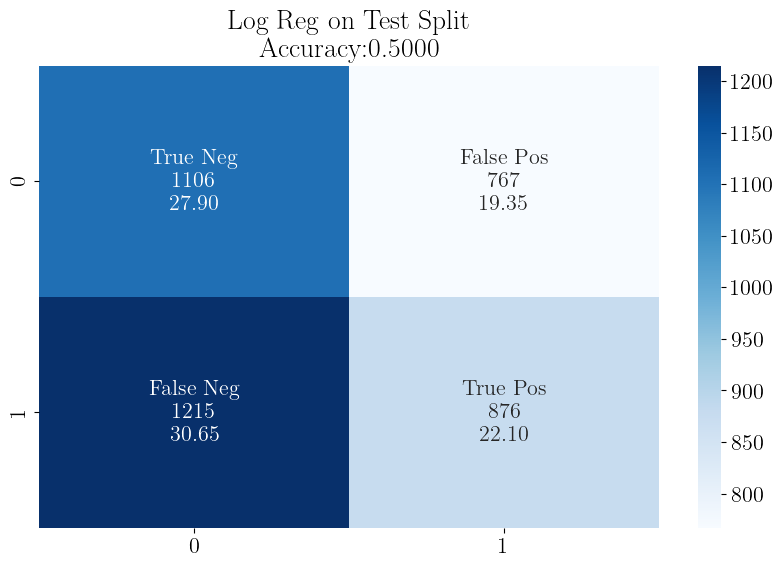
\includegraphics[width=\columnwidth]{log_reg.png}
  \caption{Logistic Regression Confusion Matrix}
  \label{fig:log_reg}
\end{figure}

\begin{figure}
  \centering
  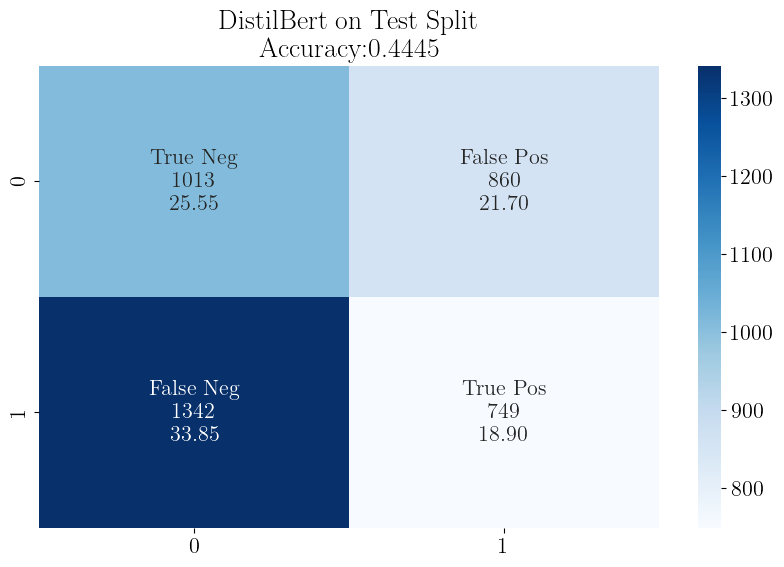
\includegraphics[width=\columnwidth]{distil.png}
  \caption{DistilBERT Confusion Matrix}
  \label{fig:distil}
\end{figure}

\section{Related Work}

\subsection{BERT Related Work}
\vspace{.5em}

\begin{itemize}
    \item\textbf{Title:} Aligning AI With Shared Human Values \\
    \textbf{Citation:} \cite{hendrycks2023aligning} \\
    \textbf{Description:} This is the paper which originated the ETHICS dataset and inspired a lot of this project - to a large extent all I'm trying to do is extend their work slightly. They focus almost entirely on BERT based approaches, especially RoBERTa (see below), so I hope that by taking advantage of improvements in BERTology (as it where) and by introducing LLMs I can make some meaningful improvements to their work.
    
    \item\textbf{Title:} Scruples: A Corpus of Community Ethical Judgments on 32,000 Real-Life Anecdotes \\
    \textbf{Citation:} \cite{lourie2021scruples} \\
    \textbf{Description:} This is a potential source of additional data, which is especially important since I seem to be having finetuning problems. These "Community Judgements" are also sourced from reddit.com/r/AMITAH, so they should dovetail well with the ETHICS dataset.

    \item\textbf{Title:} RoBERTa: A Robustly Optimized BERT Pretraining Approach \\
    \textbf{Citation:} \cite{liu2019roberta} \\
    \textbf{Description:} This paper describes many of the finetuning techniques used by Hendrycks et al. to achieve their best performance on ETHICS, so I'm hoping that I can use RoBERTa, and their finetuning techniques more broadly, to improve my abysmall current DistilBERT accuracy.
\end{itemize}

\subsection{LLM Related Work}

\begin{itemize}
    \item\textbf{Title:} The Moral Integrity Corpus: A Benchmark for Ethical Dialogue Systems\\
    \textbf{Citation:} \cite{ziems2022moral} \\
    \textbf{Description:} I'll admit, this paper is more for me than for this project specifically. They propose a Seq-Seq moral reasoning process/prompt engineering technique which injects essentially attacks on the LLM's moral reasoning in the form of sentences like "You should not judge people negatively based on race" to test and improve output. I'm still not sure if any output beyond classification from Llama is going to play a role in my final product, but if so I do think there are some valuable insights here. 

    \item\textbf{Title:} Language Models are Few-Shot Learners\\
    \textbf{Citation:} \cite{brown2020language} \\
    \textbf{Description:} This paper describes a variety of techniques for adapting LLM's Seq-Seq functioning for other tasks including text classification. This is more or less the paper on doing so, so it should be helpful as I move into the third stage of the project.
\end{itemize}

\section{Timeline}

I plan to hold to the following rough timeline of tasks:

\begin{table}[htbp]
    \centering
    \begin{tabular}{p{0.4\columnwidth} p{0.4\columnwidth}}
        \toprule
        \textbf{Task} & \textbf{Estimated Completion} \\
        \midrule
        Install Llama-2-7b, begin fine tuning & 3/29 \\
        \midrule
        Tune Additional BERT models & 4/4 \\
        \midrule
        Determine best model for web integration & 4/11 \\
        \midrule
        Implement "Digital Socrates" page & 4/16 \\
        \midrule
        Complete presentation & 4/20 \\
        \midrule
        Complete report & 4/28
        \bottomrule
    \end{tabular}
    \caption{Timeline}
    \label{tab:task_completion}
\end{table}

With some expected slop and slippage here and there.

\bibliography{references}
\bibliographystyle{acl_natbib}


\end{document}
